\documentclass{beamer}

\usepackage{amsmath}
\usepackage[style=alphabetic,url=true]{biblatex}
\usepackage{environ}
\usepackage{geometry}
\usepackage{graphicx}
\usepackage{amsmath}
\usepackage{amsfonts}
\usepackage{amssymb}
\usepackage{calrsfs}
\usepackage{listings}
\usepackage{tikz}
\usepackage[T2A]{fontenc}
\usepackage[utf8]{inputenc}
\usepackage[cache=false]{minted}

\graphicspath{ {./graphics/} }
\usetikzlibrary{shapes.arrows,chains}
\usecolortheme{beaver}
\setbeamertemplate{itemize item}[circle]
\setbeamertemplate{itemize subitem}{--}
\addtobeamertemplate{navigation symbols}{}{
  \usebeamerfont{footline}
  \usebeamercolor[fg]{footline}
  \hspace{1em}
  \insertframenumber/\inserttotalframenumber
}
\setminted[Lisp]{
  fontsize=\scriptsize
}
\setminted[text]{
  fontsize=\scriptsize
}
\usemintedstyle{xcode}
\BeforeBeginEnvironment{minted}{\medskip}
\AfterEndEnvironment{minted}{\medskip}



\title{
  Common Lisp and Introduction to Functional Programming \\
  Lecture 8: Functional Data Structures 1/2
}
\author{Yuri Zhykin}
\date{Apr 8, 2021}

\begin{document}

\frame{\titlepage}

\begin{frame}[fragile]
  \frametitle{Avoiding Explicit Mutable State 1/2}
  \begin{itemize}
  \item \textbf{Lexical bindings} allow to avoid assignment operations and
    provide a cleaner way of maintaining \textbf{local} state.
  \item \textbf{Recursion and TCO} allow to define iterative processes in a
    stateless way, replacing state with function arguments.
  \item Generally, in a lot of cases explicit state can be replaced with
    function arguments:
    \begin{itemize}
    \item this way, functions remain mathematical functions, as they still
      depend solely on their arguments (the goal),
    \item state has a clearly defined ``flow'' through the program and can be
      viewed as data.
    \end{itemize}
  \end{itemize}
\end{frame}

\begin{frame}[fragile]
  \frametitle{Avoiding Explicit Mutable State 2/2}
  \begin{itemize}
  \item Example:
\begin{minted}{Lisp}
  (defun fib-1 (n)
    (if (or (= n 0) (= n 1))
        n
        (+ (fib (- n 1)) (fib (- n 2)))))

  (defun fib-2 (n)
    (let ((a 0)
          (b 1))
      (loop 
        while (> n 0)
        do (multiple-value-setq (a b) (values b (+ a b)))
           (decf n))
      a))

  (defun fib-3 (n)
    (labels ((%fib (n a b)
               (if (= n 0)
                   a
                   (%fib (- n 1) b (+ a b)))))
      (%fib n 0 1)))
\end{minted}
  \end{itemize}
\end{frame}

\begin{frame}[fragile]
  \frametitle{Data Structures}
  \begin{itemize}
  \item \textbf{Data structure} is
    \begin{itemize}
    \item a collection of values,
    \item the relationships among these values,
    \item the functions or operations that can be applied to the data.
    \end{itemize}
  \item Data structures store state in a \textbf{semi-implicit} way: it is not
    immediately obvious that a data structure contains components that are
    modified.
  \end{itemize}
\end{frame}

\begin{frame}[fragile]
  \frametitle{Mutable Data Structures}
  \begin{itemize}
  \item Generally, most useful data structures available in modern programming
    languages are \textbf{mutable} for \textbf{efficiency reasons}.
  \item \textbf{Mutable data structure} is a data structure that can be modified
    in-place by its operations.
  \item Operations that modify the data structure in-place are called
    \textbf{destructive operations} - they ``destroy'' the existing data
    structure and replace it in memory with the new structure.
  \end{itemize}
\end{frame}

\begin{frame}[fragile]
  \frametitle{Immutable Data Structures 1/2}
  \begin{itemize}
  \item \textbf{Immutable data structure} or \textbf{persistent data structure}
    is a data structure that preserves the previous version of itself when
    modified.
  \item \textbf{Mutable data structure operations} return only the relevant
    results, while all required state changes are performed in-place in the data
    structure object.
  \item \textbf{Immutable data structure operations} return both the relevant
    results and the new version of the data structure that contains the new
    version of internal data.
  \item The old version of the data structure remains intact for any parts of
    the program that hold the reference to it.
  \end{itemize}
\end{frame}

\begin{frame}[fragile]
  \frametitle{Immutable Data Structures 2/2}
  \begin{itemize}
  \item Advantages:
    \begin{itemize}
    \item no need to track which program components modify the data structure -
      the new versions of the structure are created by its operation, returned
      as results and propagated through the program,
    \item programs that work with immutable data structures are trivially
      \textbf{parallelizable}.
    \end{itemize}
  \item Drawbacks:
    \begin{itemize}
    \item new version of the data structure is \textbf{a copy} of the previous
      object with some modifications, the old object still takes memory,
    \item copying the data structure on every operations consumes a lot of
      memory,
    \item this approach relies heavily on efficient \textbf{memory management}
      and \textbf{garbage collection}.
    \end{itemize}
  \end{itemize}
\end{frame}

\begin{frame}[fragile]
  \frametitle{Copy-on-Write}
  \begin{itemize}
  \item \textbf{Copy-on-write} (\textbf{CoW}) approach distinguishes between
    \textbf{read} and \textbf{write} operations and is based on the following
    idea
    \begin{itemize}
    \item if a part of the structure is only being \textbf{read}, it can be
      shared between multiple readers,
    \item if a part of the structure is modified, a new of the structure is
      created with all the parts \textbf{except} the one being \textbf{written}
      shared with the original structure,
    \item the new copy of structure is than modified in-place with no effect on
      the original structure.
    \end{itemize}
  \end{itemize}
\end{frame}

\begin{frame}[fragile]
  \frametitle{Structure Sharing}
  \begin{itemize}
  \item \textbf{Structure sharing} is an approach to implementing immutable data
    structures that partially resolves the problem of memory consumption.
  \item \textbf{Structure sharing} is a variant of the \textbf{CoW}: we only
    need to copy the parts of the data structure that are being modified.
  \item If \textbf{structure sharing} is implemented for primitive data
    structures provided by the language, more complex data structures can be
    constructed from the primitive ones in a way that preserves structure
    sharing benefits.
  \end{itemize}
\end{frame}

\begin{frame}[fragile]
  \frametitle{Common Lisp's Lists 1/2}
  \begin{itemize}
  \item \textbf{Common Lisp's list} is one of the simplest examples of
    structure sharing:
\begin{minted}{Lisp}
  CL-USER> (setf list-1 (list 1 2 3))
  (1 2 3)
  CL-USER> (setf list-2 (cons 0 list-1))
  (0 1 2 3)
  CL-USER> list-1
  (1 2 3)
  CL-USER> (eq (cdr list-2) list-1)
  T
  CL-USER> (setf list-3 (list 'a (list 'b 'c)))
  (4 5 6)
  CL-USER> (setf list-4 (append list-3 list-1))
  (a (b c) 1 2 4)
  CL-USER> (eq (cdr (cdr (cdr list-4) list-1)))
  T
\end{minted}
  \end{itemize}
\end{frame}

\begin{frame}[fragile]
  \frametitle{Common Lisp's Lists 2/2}
  \begin{itemize}
  \item Internal representation:
\begin{minted}{text}
           +---+   +---+   +---+            
   list-3: | a |-->| * |-->|NIL|            
           +---+   +--\+   +---+            
                       \
                        \+---+   +---+   +---+
                         | b |-->| c |-->|NIL|
                        /+---+   +---+   +---+
                       /  
           +---+   +--/+
   list-4: | a |-->| * |
           +---+   +--\+ 
                       \
                        \+---+   +---+   +---+   +---+
   list-1:               | 1 |-->| 2 |-->| 3 |-->|NIL|
                        /+---+   +---+   +---+   +---+
                       /      
                +---+ /
   list-2:      | 0 |/
                +---+   
\end{minted}
  \end{itemize}
\end{frame}

\begin{frame}[fragile]
  \frametitle{Building on Lists: 1/4}
  \begin{itemize}
  \item Lists are great at representing sequences, but can we use them to
    represent associative maps (associative arrays or key-value structures)?
  \item \textbf{P-lists} (\textbf{plists}, \textbf{property lists}) are lists
    that store keys and values in a flat structure:
\begin{minted}{Lisp}
    CL-USER> (setf plist '(:a 1 :b 2 :c 3))
    (:a 1 :b 2 :c 3)
    CL-USER> (getf plist :b)
    2
    CL-USER> (setf (getf plist :b) 22) ;; destructive
    22
    CL-USER> plist
    (:a 1 :b 22 :c 3)
\end{minted}
  \end{itemize}
\end{frame}

\begin{frame}[fragile]
  \frametitle{Building on Lists 2/4}
  \begin{itemize}
  \item \textbf{A-lists} (\textbf{alists}, \textbf{associative lists}) are lists
    that store keys and values as \mintinline{Lisp}{cons}-pairs:
\begin{minted}{Lisp}
    CL-USER> (setf alist '((:a . 1) (:b . 2) (:c . 3)))
    ((:a . 1) (:b . 2) (:c . 3))
    CL-USER> (assoc :b alist)
    (:b . 2)
    CL-USER> (setf (cdr (assoc :b alist)) 22) ;; destructive
    22
    CL-USER> alist
    ((:a . 1) (:b . 22) (:c . 3))
\end{minted}
  \end{itemize}
\end{frame}

\begin{frame}[fragile]
  \frametitle{Building on Lists: 3/4}
  \begin{itemize}
  \item \textbf{Associative lists} can be easily adapted to be functional data
    structures (i.e. update operations can be implemented in a non-destructive
    manner).
  \item \textbf{Problem with associative lists} is that they are very
    inefficient in general:
    \begin{itemize}
    \item lookup operations take $O(n)$ time, where $n$ is the number of
      elements in the list,
    \item update operations take $0(n)$ time and $0(n)$ space in the worst case
      scenario,
    \item for comparison, both lookup and update operations on a mutable
      \mintinline{Lisp}{hash-table} take $O(1)$ time (update also takes $0(1)$
      space on average).
    \end{itemize}
  \end{itemize}
\end{frame}

\begin{frame}[fragile]
  \frametitle{Building on Lists: 4/4}
  \begin{itemize}
  \item Can we have \mintinline{Lisp}{hash-table}-like performance on an
    immutable data structure?
  \item The answer is \textbf{trees}.
  \item \textbf{Clojure} language heavily relies on structure-sharing trees
    implementation for most of its primitive data structures.
  \item In \textbf{Common Lisp}, structure-sharing trees can be easily
    implemented on top of built-in structure-sharing lists.
  \end{itemize}
\end{frame}

\begin{frame}[fragile]
  \frametitle{Useful Resources}
  \begin{minipage}{0.6\textwidth}\raggedright
    \begin{itemize}
    \item \textbf{Purely Functional Data Structures} by Chris Okasaki
    \end{itemize}
  \end{minipage}
  \begin{minipage}{0.3\textwidth}
    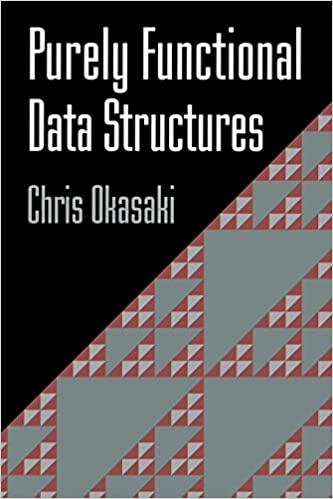
\includegraphics[width=\linewidth]{pfds}
  \end{minipage}
\end{frame}

\begin{frame}
  \frametitle{The End}
  \begin{center}
    Thank you!
  \end{center}
\end{frame}

\end{document}

%%% Local Variables:
%%% mode: latex
%%% TeX-master: t
%%% TeX-command-extra-options: "-shell-escape"
%%% End:
